\documentclass[10pt,a4paper,oneside]{book}
\usepackage[utf8]{inputenc}
\usepackage[spanish]{babel}
\usepackage{amsmath}
\usepackage{amsfonts}
\usepackage{amssymb}
\usepackage{graphicx}
\usepackage[left=2cm,right=2cm,top=2cm,bottom=2cm]{geometry}
\usepackage{hyperref}
\usepackage{wrapfig}
\hypersetup{
    colorlinks=true,
    linkcolor=cyan,
    anchorcolor=cyan,
    filecolor=cyan,
    urlcolor=blue,
}

%Header and footer customized
\usepackage{fancyhdr}
\pagestyle{fancy}

\usepackage{xcolor}
\usepackage{titling}

\usepackage{listingsutf8}
\usepackage{listings}
\usepackage{color}


%New colors defined below
\definecolor{codegreen}{rgb}{0,0.6,0}
\definecolor{codegray}{rgb}{0.5,0.5,0.5}
\definecolor{codepurple}{rgb}{0.58,0,0.82}
\definecolor{backcolour}{rgb}{0.95,0.95,0.92}

%Code listing style named "mystyle"
\lstdefinestyle{mystyle}{
  backgroundcolor=\color{backcolour},   commentstyle=\color{codegreen},
  keywordstyle=\color{magenta},
  numberstyle=\color{codegray},
  stringstyle=\color{codepurple},
  basicstyle=\scriptsize\ttfamily\tiny,
  breakatwhitespace=false,         
  breaklines=true,                 
  captionpos=b,                    
  keepspaces=true,                                     
  numbersep=5pt,                  
  showspaces=false,                
  showstringspaces=false,
  showtabs=false,                  
  tabsize=2,
  framextopmargin=1pt,
  framexbottommargin=10pt,
}

\usepackage{sectsty}
\partfont{\large}

%"mystyle" code listing set
\lstset{style=mystyle}

%For generate graphs
\usepackage{pgf}
\usepackage{tikz}
\usetikzlibrary{arrows,automata}

% To generate a box with text and background
\definecolor{shadecolor}{RGB}{200,201,190}
\newcommand{\mybox}[1]{\par\noindent\colorbox{shadecolor}
{\parbox{\dimexpr\textwidth-2\fboxsep\relax}{#1}}}

\author{Ruben Vasallo Gonzalez}
\title{PROYECTO FINAL MÁSTER \\ CLASIFICADOR DOCUMENTOS MÉDICOS HOPE \\ 2020 - 2021}

%header
\headsep = 1,5cm
\lhead{\begin{picture}(0,0) \put(0,0){
\includegraphics[width=2cm]{logo-uoc-default.png}} \end{picture}}
\chead{}
\rhead{\thetitle \\ \theauthor}

%footer
\lfoot{}
\cfoot{\thepage}
\rfoot{}

%set head of page
\setlength{\textheight}{230mm}

\begin{document}
\maketitle

\tableofcontents

\chapter{Presentación del Máster}

\section{Definición del proyecto}

\paragraph{}
El proyecto de fin de máster que aquí se presenta nace de la necesidad por parte del \textit{proyecto HOPE} de clasificar y recomendar resultados sobre estudios clínicos de confianza y que estén actualizados. En Internet existe muchísima información sobre medicina y salud y no siempre toda es de fiar.

\paragraph{}
El proyecto HOPE (que significa \textit{Health Operations for Personalized Evidence} en ingles) nace de la necesidad de ayudar a los científicos médicos a encontrar la información que necesitan de la manera más rápida y fácil posible. Existe infinidad de información medica en Internet de miles de proyectos de investigación medica y esto hace que, muchas veces sea complicado encontrar la información sobre ensayos médicos para tratar información. En el ámbito de la medicina el tiempo perdido puede costar vidas y es un precio demasiado elevado a pagar, tanto a nivel económico como emocional.

\paragraph{}
Actualmente existen bases de datos de confianza en donde los científicos y el publico en general puede buscar informes y ensayos sobre estudios clínicos desarrollados anteriormente, pero no siempre es fácil o rápido encontrar estos resultados.

\paragraph{}
El proyecto HOPE es un sistema basado en inteligencia artificial para identificar los datos claves de casos clínicos registrados en la Historia Clínica Electrónica, en base a los cuales realiza una búsqueda única por paciente para proporcionar al profesional de la salud recomendaciones de tratamientos, estudios de investigación, información para el paciente, todo en base a registros de fuentes científicas de información. En este proyecto, médicos de todo el mundo puede consultar en una base de datos informes médicos relacionados con los síntomas que puedan tener sus pacientes y ver que otros tratamientos han dado resultado. Todo y con eso, el sistema no siempre devuelve los artículos más relevantes o actualizados por lo que, no siempre la información consultada es útil.

\paragraph{}
En este ámbito, los profesionales médicos pueden valorar si la información recibida ha sido útil o no respecto a la búsqueda que han realizado, por lo que con ese \textit{feedback}, se pretende mejorar el sistema actual complementándolo con un modelo clasificador capaz de ayudar al actual a entregar realmente los artículos útiles basándose en el \textit{feedback} que los médicos dan al sistema.

\chapter{Objetivos del Máster}

\section{Objetivo principal}

\paragraph{}
El objetivo principal que se pretende alcanzar en este proyecto es el de entrenar un modelo predictivo de tipo clasificador que sea capaz de discriminar en base a los términos buscados por el medico, cuales son los artículos más útiles que pueden ayudar en el tratamiento del paciente.

\paragraph{}
Este modelo predictivo tendrá que ser capaz de clasificar si un documento/articulo que esta relacionado un unas \textit{Keywords} y unos términos (dolencias) buscados por un usuario sera útil o no para este usuario. Esto permitirá a los médicos poder consultar de una manera inmediata la información de otras pruebas relacionadas con las dolencias del paciente y así poder decidir aplicar o no las mismas pruebas. Ademas también permitirá que pacientes que aparentemente no tenían un tratamiento disponible para la dolencia que tiene y que están en cuidados paliativos, puedan probar posibles tratamientos relacionados con las dolencias que tienen, y que si han funcionado en otros pacientes.

\paragraph{}
Con todo esto, el entregable final sera el código necesario para crear y ejecutar el modelo predictivo que mejor acierto tenga con el dataset facilitado para poder realizar el entrenamiento y pruebas de la validación del modelo.

\section{Objetivos secundarios}

\paragraph{}
Debido a que la creación de un modelo predictivo funcional es un primer paso fundamental para solucionar el problema, el propio modelo en si no servirá de nada si no existe una manera útil y sencilla de poder usarlo.

\paragraph{}
Por eso, si se consigue entrenar un modelo lo suficientemente útil para que de resultados correctos, se plantea como objetivo secundario el crear una interfaz (api REST) que facilite el uso de este modelo.

\paragraph{}
Esta api deberá recoger por parámetro los atributos necesarios para que el modelo se pueda ejecutar y devuelva la respuesta de si el articulo es valido o no

\chapter{Metodología}

\section{Extracción de los datos}

\paragraph{}
El Origen de los datos se encuentra en una Base de datos SQL distribuida en dos tablas, que pasamos a detallar a continuación:

\paragraph{• Tabla \textit{fed\_hope\_sugerencia}}

\paragraph{}
\begin{figure}[!htb]
  \centering
  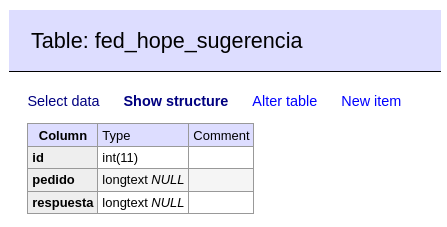
\includegraphics[width=8cm]{images/metodologia_tabla_fed_hope_sugerencia.png}
  \caption{Visualización de los atributos de la tabla \textit{fed\_hope\_sugerencia}}
\end{figure}

\paragraph{}
En esta tabla encontraremos la sugerencia que dio el programa HOPE en base a los parámetros que introdujo el usuario, almacenado en el atributo pedido y la respuesta que dio el programa, almacenado en el atributo respuesta. Todos los datos son almacenados en formato documento json.

\newpage
\paragraph{\textbf{Atributo pedido}: } Si analizamos el formato de datos que tenemos del atributo pedido observamos los siguientes atributos:

\lstset{inputencoding=utf8/latin1}
\lstinputlisting[frame=single]{codes/metodologia_tabla_fed_hope_sugerencia_attribute_pedido.json}

\paragraph{}
Podemos ver varios atributos haciendo referencia a los síntomas que consulta el profesional medico.

\paragraph{\textbf{Atributo respuesta}: } En el atributo respuesta obtenemos entre otros datos, el listado de artículos científicos sugeridos relacionados con los síntomas descritos por el profesional medico. Esta respuesta es muy amplia pero entre todos los atributos, podemos observar un listado de identificadores de artículos, con sus fechas de revisión de estos, y unas palabras claves descriptivas para esos artículos.

\paragraph{}
\textbf{Nota:} Mostramos una pequeña parte del contenido de una observación del atributo respuesta.
\begin{figure}[!htb]
  \centering
  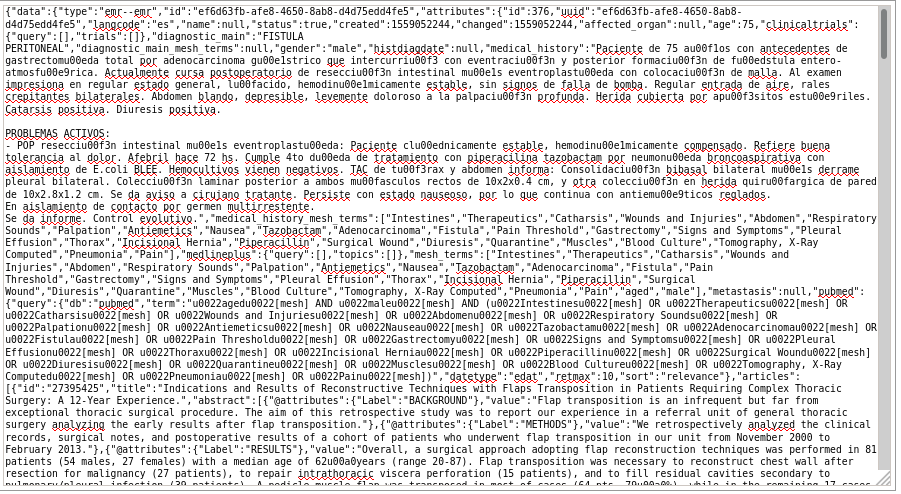
\includegraphics[width=15cm]{images/metodologia_tabla_fed_hope_sugerencia_attribute_respuesta.png}
  \caption{Ejemplo de contenido del atributo respuesta de una observación}
\end{figure}

\newpage
\paragraph{• Tabla \textit{fed\_hope\_sugerencia\_feedback}}

\paragraph{}
\begin{figure}[!htb]
  \centering
  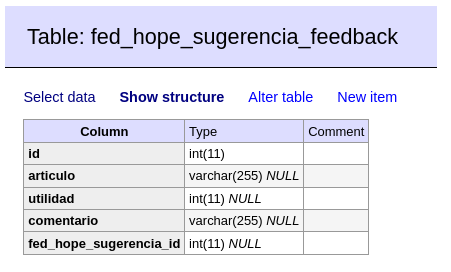
\includegraphics[width=8cm]{images/metodologia_tabla_fed_hope_sugerencia_feedback.png}
  \caption{Visualización de los atributos de la tabla \textit{fed\_hope\_sugerencia\_feedback}}
\end{figure}

\paragraph{}
En esta tabla encontraremos la opinión \textit{feedback} (que utilidad ha tenido la información por parte del usuario) de la información recibida dado un articulo en concreto en una búsqueda en concreto. Esta información se relaciona con la tabla \textit{fed\_hope\_sugerencia} a través del atributo \textit{fed\_hope\_sugerencia\_id}.

\paragraph{}
En esta tabla esta representada la opinión \textit{feedback} del usuario en el atributo \textit{utilidad}, que denota un valor 0 para los artículos que han sido poco útiles respecto a la búsqueda realizada y 1 para los artículos que si han sido útiles.

\newpage
\subsection{Lectura de los datos de MySQL}

\paragraph{}
El primer paso sera extraer de la base de datos \textit{MySQL} el dataset de datos. Para realizar esta acción nos ayudaremos de las librerías \textit{sqlalchemy} y \textit{pymysql} programadas en lenguaje \textit{python} que nos permitirá acceder a la información almacenada en una base de datos \textit{MySQL} y devolvérnosla en formato \textit{dataframe}, un formato que nos permite entre otras cosas, realizar transformaciones de los datos para conseguir nuestro objetivo final.

\paragraph{}
Este formato es interpretable por la librería \textit{pandas} y \textit{numpy}, dos librerías programadas en lenguaje \textit{python}, muy comunes en el ámbito de la ciencia del dato, que nos facilitara entre otras cosas, poder hacer operaciones matemáticas con los datos de manera eficiente.

\paragraph{}
\begin{figure}[!htb]
  \centering
  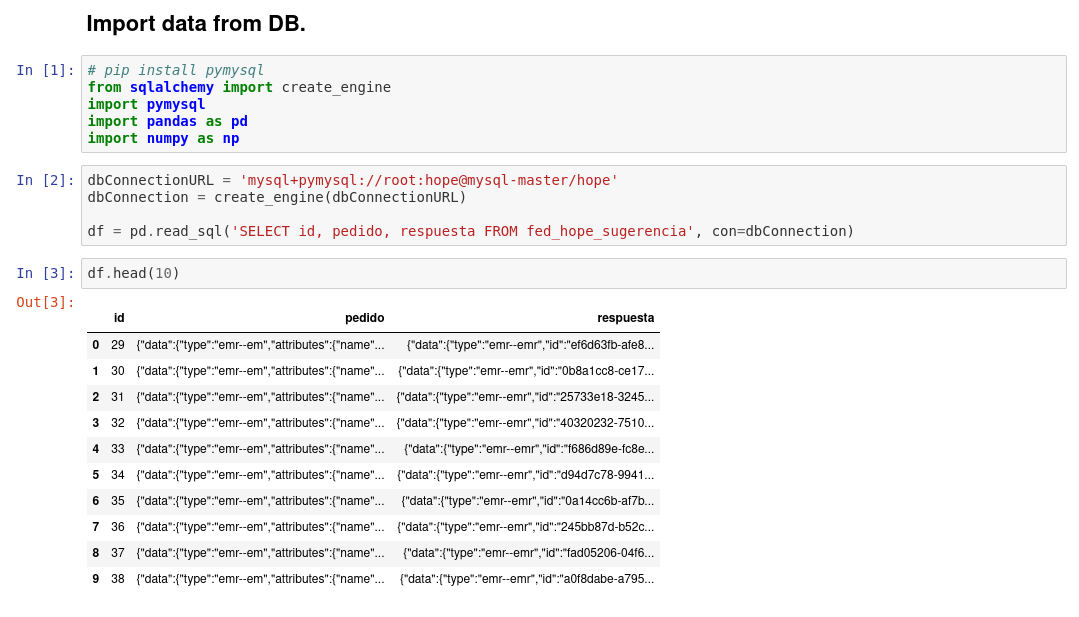
\includegraphics[width=0.9\textwidth]{images/metodologia-extract-data-mysql.png}
  \caption{Lectura de los datos de Mysql}
\end{figure}

\newpage
\subsection{Conversión a formato columnar}

\paragraph{}
Para poder trabajar con los datos, necesitaremos que estos estén en formato columnar (tabla relacional) por lo que necesitaremos convertir los datos de estos \textit{json} en tablas relacionales (A esta acción se le conoce como \textit{flattening} o aplanar). 

\paragraph{}
Este paso consiste en coger cada uno de los atributos que tiene el json y convertirlos en columnas de una tabla, añadiendo los valores. Si el \textit{json} tiene varios niveles, este proceso añadirá tantas columnas como niveles tenga el \textit{json}, siempre que todas las observaciones del \textit{json} tengan el mismo formato. Este caso se nos cumple para las observaciones del atributo Pedido. No es así para las observaciones del atributo respuesta en el que tendremos que hacer un tratamiento especial que detallaremos posteriormente.

\paragraph{}
Para poder realizar esta acción, primero tendremos que solucionar un problema de tratamiento de texto. Los datos que se nos proporcionan, contienen caracteres que informan de un salto de linea o tabulador. Estos caracteres pueden ser mal interpretados a la hora de leer los datos de los documentos en formato \textit{json} por lo que los eliminaremos de los datos (substituyendo-los por espacios vacíos).

\paragraph{}
\begin{figure}[!htb]
  \centering
  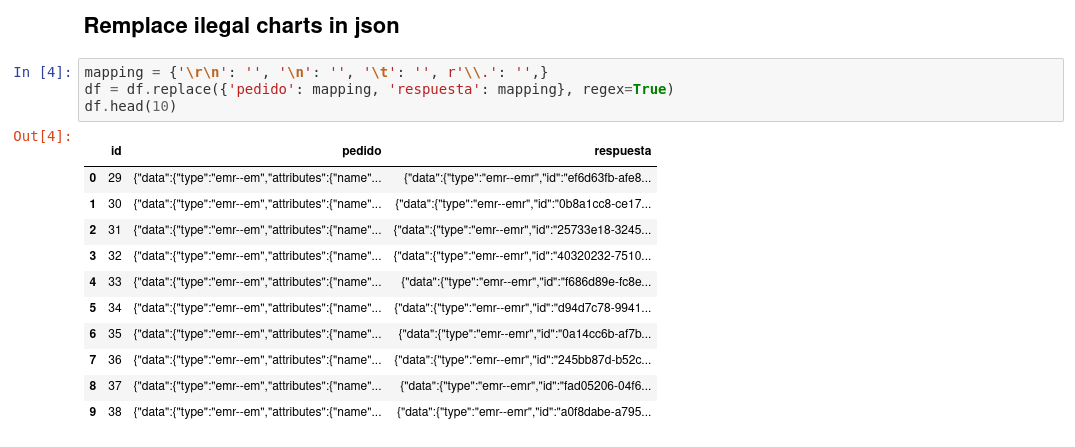
\includegraphics[width=0.9\textwidth]{images/metodologia-eliminar-caracteres-prohibidos.png}
  \caption{Eliminación de caracteres erróneos.}
\end{figure}

\newpage
\paragraph{• \textit{Flattening} del atributo pedido}

\paragraph{}
Para realizar la acción de \textit{flattening} en el atributo pedido, nos ayudaremos de la funcionalidad \textit{json\_normalize} del paquete pandas que realiza esta acción. 

\paragraph{}
\begin{figure}[!htb]
  \centering
  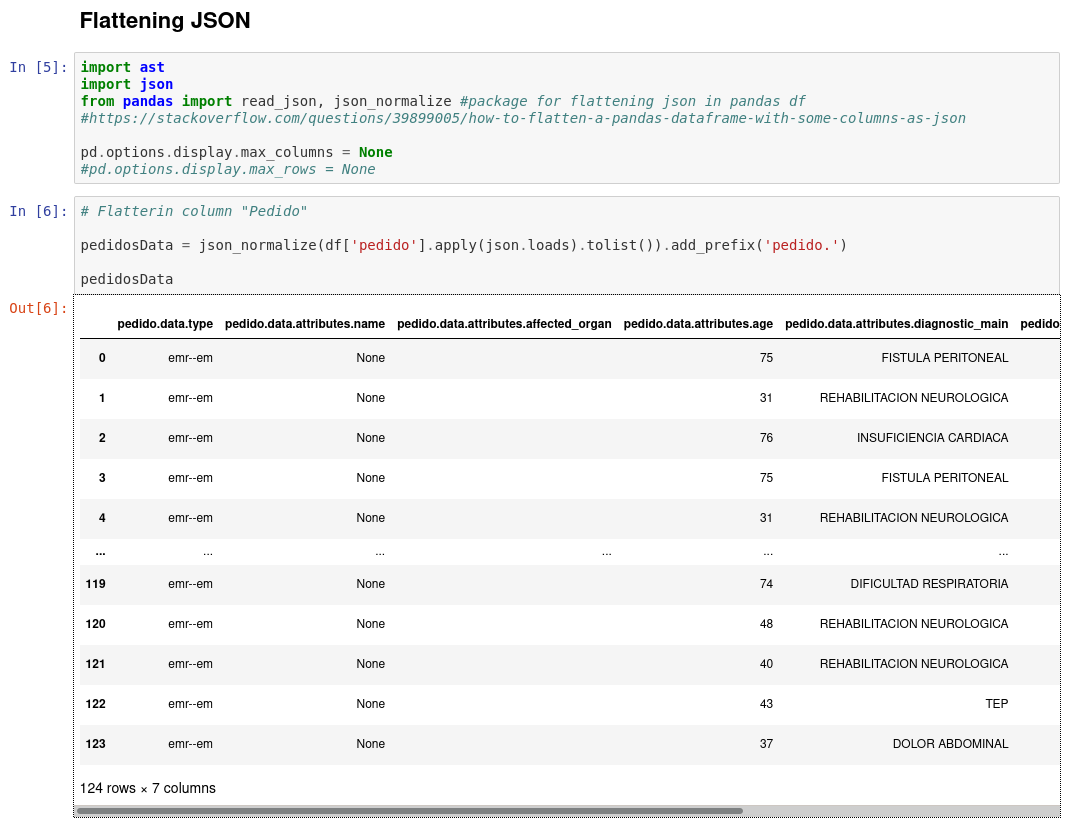
\includegraphics[width=0.9\textwidth]{images/metodologia-aplanar-pedido.png}
  \caption{\textit{Flattening} del atributo pedido.}
\end{figure}

\paragraph{• \textit{Flattening} del atributo respuesta}

\paragraph{}
Debido a que la información almacenada en el documento \textit{json}, en el atributo respuesta es muy compleja (debido a que esta contiene diferentes documentos con diferentes niveles de información) como se puede apreciar en el apartado X, no podemos aplanar la información directamente como hemos hecho con el atributo pedido. Por lo que tenemos que analizar que información nos interesa recoger para enriquecer el dataset de datos.

\paragraph{}
Después de analizar el documento, y ayudarnos del conocimiento del cliente, vemos que los atributos más interesantes son los que hacen referencia al identificador del articulo, las palabras claves asociadas al articulo por parte de la api pubmed y el mes y año de la revisión del articulo.

\paragraph{}
\begin{figure}[!htb]
  \centering
  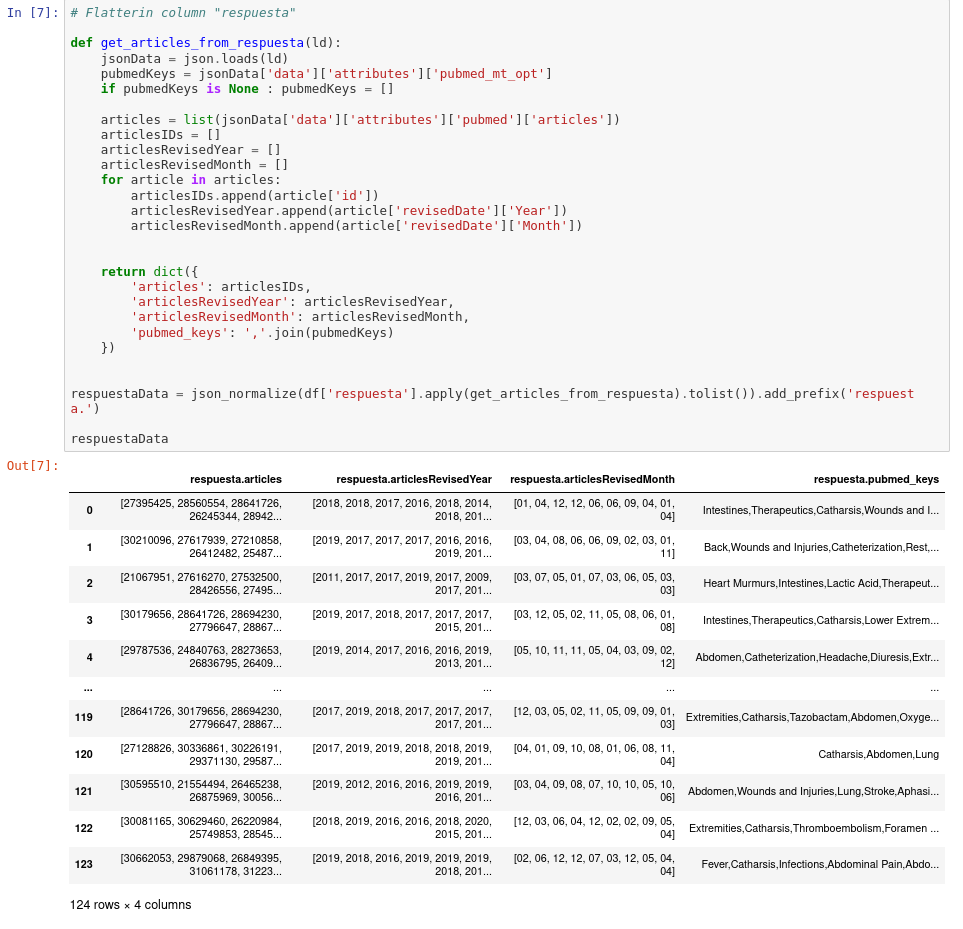
\includegraphics[width=0.9\textwidth]{images/metodologia-aplanar-respuesta.png}
  \caption{\textit{Flattening} del atributo respuesta.}
\end{figure}



\newpage
\section{Procesado de los datos}
TODO

\section{Análisis de los datos}

\subsection{Análisis de componentes principales}
TODO

\section{Enriquecimiento de los datos. Aproximación por Vecinos más próximos (K-NN)}
TODO

\section{Modelos Predictivos}

\subsection{Regresión logística}
TODO

\chapter{Conclusiones}

\section{Resultados obtenidos}
TODO

\end{document}